% !TEX root = ../thesis.tex
\chapter{Simulation studies}
\section{Assumptions}
The general setting described in section \ref{solution} is simplified in the
rest of this work by assuming:
\begin{itemize}
	\item[--] same domain for all the patients, \ie
		$\Omega_1 = \ldots = \Omega_m:= \Omega$;
	\item[--] same locations
		$\bm{p}_{ij}$ for every patient $i$, that is $\bm{p}_{ij}=\bm{p}_{kj} \quad
			\forall (i,k) \in \{ 1 \ldots m \}^2$. This also implies that $n_i$, number
		of observations for patient $i$, is the same for every $i$. In the following
		we will use $n=n_i$.
	\item[--] same finite element basis used across all $m$
		domains $\Omega$ ($N_{\tau}= m \times n$).
		%	\item[--]
		%		\listvalues
\end{itemize}
These properties allow storing in memory some of the matrices
described above just for one patient rather than for all patients. In the
problems where assumptions above are valid but some data are missing, as it
happens in concrete cases, some adjustments are necessary. The treatment is
analogous to the one for the basic spatial regression case described in
appendix \ref{secNA}. In fact, in theory the mixed-effects model is not
distinguishable from a model in which the random effects have been treated as
different covariates for each unit.

To treat missing values the following adjustments are therefore sufficient:
\begin{itemize}
	\item[--] replace the missing values with $0$;
	\item[--] replace the covariates corresponding to the missing value with $0$s;
	\item[--] replace the rows of $\tilde{\Psi}$ matrix corresponding to the
		missing value with $0$s.
\end{itemize}

We make a comparative study on the performance of the iterative method, with
respect to solving the monolithic matrix. Several cases are considered in the
following sections.

From an implementative point of view, I have extended the capabilities of the
version of the library implemented by \citeauthor{kim}, who in turn developed a
branch of the \texttt{fdaPDE} package available on \texttt{CRAN}. Her branch is
called \texttt{fdaPDE\_mixed}, while my code is available on GitHub, see
\cite{MI}.

It is worth mentioning that when I began to work on this project, several new
versions of \texttt{fdaPDE} had come out, so I took the opportunity to update
the APIs that were provided by \citeauthor{kim} and refactor her code in such a
way that it will be easear to maintain a mixed-effects branch in the future.

\section{Simulations}
\subsection{Bidimensional domain}
The first case that we study is the same treated in \cite{kim}. The domain
considered is a C-shape, with a surface test function obtained from
Wood\cite{wood2008soap}, originally introduced by Ramsay
\cite{ramsay2002spline}. The C-shaped function features the property that the
inner part of the domain is close in terms of distance, yet the evaluations are
in contrast between the upper and lower sides.

In her work \citeauthor{kim} showed that the SRPDE approach leaded to results
similar to the one provided by a generalized additive model, and performed
better in terms of mean root square error concerning the spatial component of
the model.

In the simulation, we generate randomly 50 scenarios for the mixed-effects
model with 3 statistical units each. Errors $\epsilon$ are simulated as
$\mathcal{N}(0, 0.05*k)$ where $k$ is the range (difference between maximum and
minimum) of the spatial field over the observed locations. For each statistical
unit we observe 100 fixed locations, more or less uniformly on the C-shaped
domain.

The true parameter values are set to $\beta_1 = 3$, $\beta_2 = 0.5$, $b_{11} =
	-5$, $b_{21} = 0$, and $b_{31} = 5$. Covariates are generated as $sin(2\pi
	x)cos(2\pi y)$ and $N(0, 4)$, respectively. Both covariates are the same across
all statistical units.

The model estimates coefficients given a fixed grid of $\lambda$ values, and
the $\lambda$ value with the minimum generalized cross-validation (GCV) is
chosen as the best $\lambda$ from the grid.

The logic for choosing the appropiate values of the grid is the following: if
the same $\lambda$ is observed most of the times on different simulations, it
means that the grid is not fine enough near the optimal $\lambda$. Moreover the
grid of $\lambda$ should be big enough so that the boundary of the grid is not
chosen. Cleary, on the other hand, if the grid is too fine, the method would be
very slow. In practice the grid is chosen through trial and error.

Tolerance for the iterative method was chosen to be $10^{-6}$.\\ In figure
\ref{lambda} we show the comparison of the $\lambda$ selected values, the
difference is due to the different method for computing the degrees of freedom,
since the solutions are the same if not for the tolerance. Despite looking
slightly different in truth the selected values of $\lambda$ are the same if
not for a few of them where the index is shifted on the grid by one.

Figure \ref{iterations} shows how many iterations were needed for convergence
on the grid of $\lambda$. In all cases it converged very rapidly, in less than
4 iterations.

\begin{figure}[t]
	\centering
	\begin{subfigure}{0.45\textwidth}
		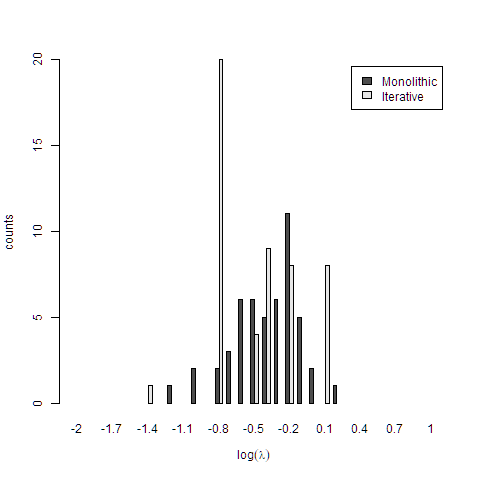
\includegraphics[width=\textwidth]{images/lambda.png}
		\centering
		\caption{\textit{Frequency of selected $\lambda$ over 50 simulations. }}
		\label{lambda}
	\end{subfigure}
	\hfill
	\begin{subfigure}{0.45\textwidth}
		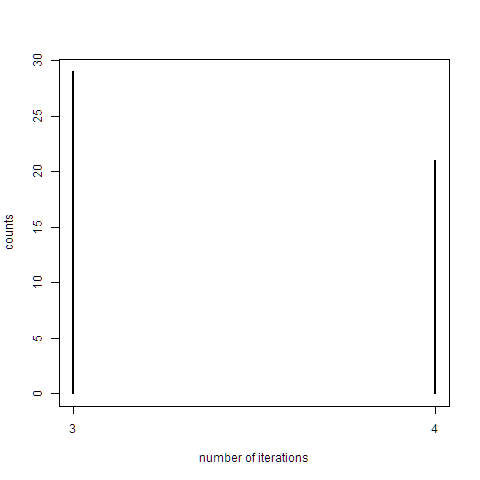
\includegraphics[width=\textwidth]{iterations.png}
		\centering
		\caption{\textit{ Iterations observed on different values of $\lambda$ }}
		\label{iterations}
	\end{subfigure}
	\begin{subfigure}{0.45\textwidth}
		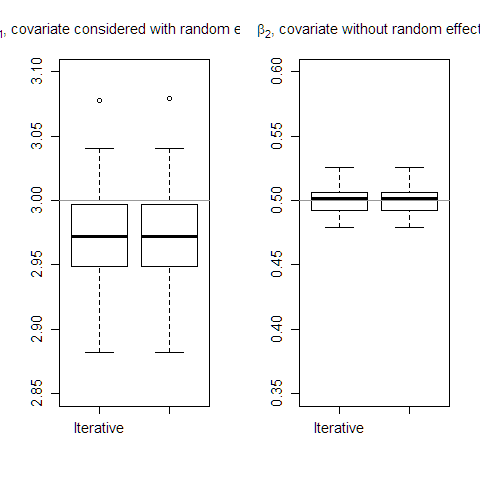
\includegraphics[width=\textwidth]{images/beta.png}
		\centering
		\caption{\textit{Boxplots for fixed effects parameters. }}
		\label{beta}
	\end{subfigure}
	\hfill
	\begin{subfigure}{0.45\textwidth}
		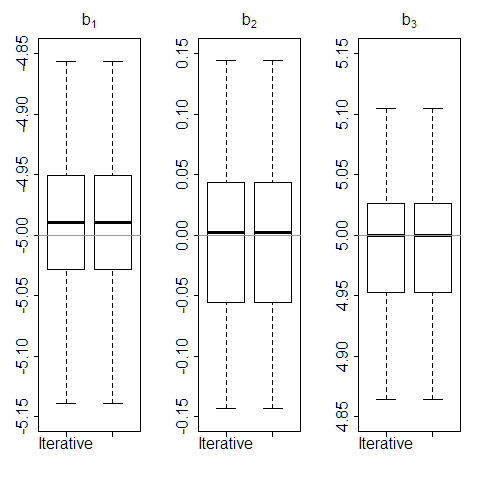
\includegraphics[width=\textwidth]{images/b.png}
		\centering
		\caption{\textit{Boxplots for random effects parameters.}}
		\label{b}
	\end{subfigure}
\end{figure}

In figure \ref{beta} we show the boxplot for the estimated $\beta_1$,
$\beta_2$, with no significant difference between the two solvers. Same goes
for figure \ref{b} for what concerns the values of $b_i$.

\begin{figure}[t]
	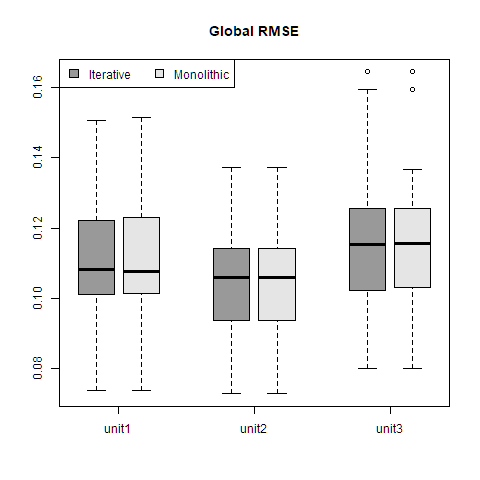
\includegraphics[width=0.6\textwidth]{images/rmse.png}
	\centering
	\caption{\textit{Root mean square error for the estimated model.}}
	\label{rmse}
\end{figure}
Finally, figure \ref{rmse} shows that there is no degradation of
performance on the global error estimated for the model.

We tried a bit varying the number of units and the number of locations and no
problems have been yet observed. However, it is important to note that the
simulation study was conducted under specific assumptions and conditions, and
the performance of the method may vary in different settings.

\subsection{Manifold domain}
aaa
\subsection{NAs handling}
discorso media It is important to note that missing data can have a significant
impact on the performance of statistical models. In the study described, the
RMSE increased with the presence of missing data in the response variable.
However, it is encouraging to see that the model was able to recover a
considerable amount of information even in the presence of missing data.

Furthermore, the study also highlighted the impact of randomness in covariates
on the performance of the model. When there was a high level of randomness in
the covariates, the model was less accurate. However, as the level of
randomness decreased, the model's accuracy improved.

Overall, the results suggest that mixed-effect models can be a useful tool for
handling missing data in real-world applications. However, it is important to
carefully consider the level of randomness in the covariates and to choose an
appropriate model based on the specific characteristics of the data.

% \begin{figure}[t] \begin{subfigure}{0.45\textwidth}
% \includegraphics[width=\textwidth]{images/1boxplot_beta1.png} \caption{}
% \label{fig:pattern1} \end{subfigure} \hfill
% \begin{subfigure}{0.45\textwidth}
% \includegraphics[width=\textwidth]{images/1boxplot_beta2.png} \caption{}
% \label{fig:pattern2} \end{subfigure}
% \caption{\textit{(\subref{fig:pattern1}) shows the pattern of generic
% symmetric matrix $X^TX$ as defined in equation~\ref{matrix:x}. Size has
% been arbitrarily chosen to be 40. On the right we show the pattern of the
% inverse of such matrix, illustrating that the inverse is dense. Non-zero
% values were sampled from a uniform distribution.}} \label{fig:pattern}
% \end{figure}
